
The Fisher-Rao metric allow us to formulate a suitable criterion for the
pairwise alignment problem, as presented in section \ref{SEC:L2PAIRWISE},
 that avoids all the problems associated with the metric $\mathbb{L}^2$.

Given $f_1, f_2 \in \mathscr{F}$, to register $f_1$ to $f_2$ the Fisher-Rao distance
will be minimized as energy term $E$ (see eqn. \ref{EQ:ENERGY}), i.e.,
the warping used in the alignment will be

\begin{equation}[EQ:DPAELASTIC]{Pairwise alignment with F-R metric}
\gamma^{*}= \operatorname{argmin}_{\gamma \in \Gamma} d_{FR}(f_1 \circ \gamma,
f_2) = \operatorname{argmin}_{\gamma \in \Gamma} \|
(q_1, \gamma) - q_2 \|_{\mathbb{L}^2}.
\end{equation}

The energy used to align the functions in figure \ref{SBFIG:PAIRWISE1} is
actually this quantity.
Since
$E[f_1, f_2] = E[f_1 \circ \gamma, f_2 \circ \gamma]$, the warping used to
register $f_1 \circ \gamma$ to $f_2 \circ \gamma$ will be the same as in the
previous case.

Because of this property, our problem will have inverse consistency, since

\begin{equation}[]{Inverse consistency}
E[f_1 \circ \gamma, f_2] = E[f_1 \circ \gamma \circ \gamma^{-1}, f_2
\circ \gamma^{-1}] = E[f_1, f_2 \circ \gamma^{-1}],
\end{equation}

so that the warping needed to register $f_2$ to $f_1$  is ${\gamma^*}^{-1}$.
In addition, the so-called pinching effect will not appear, due to the term
$\sqrt{\dot \gamma}$ that is present in the criterion to minimize.


%%, as it is shown in \ref{FIG:INVERSE}.
%\begin{figure}[Inverse consistency of pairwise alignment]{FIG:INVERSE}{Inverse consistency of pairwise alignment}
%  \subfigure[SBFIG:INVERSE1]{Alignment of $f_1$ to $f_2$}{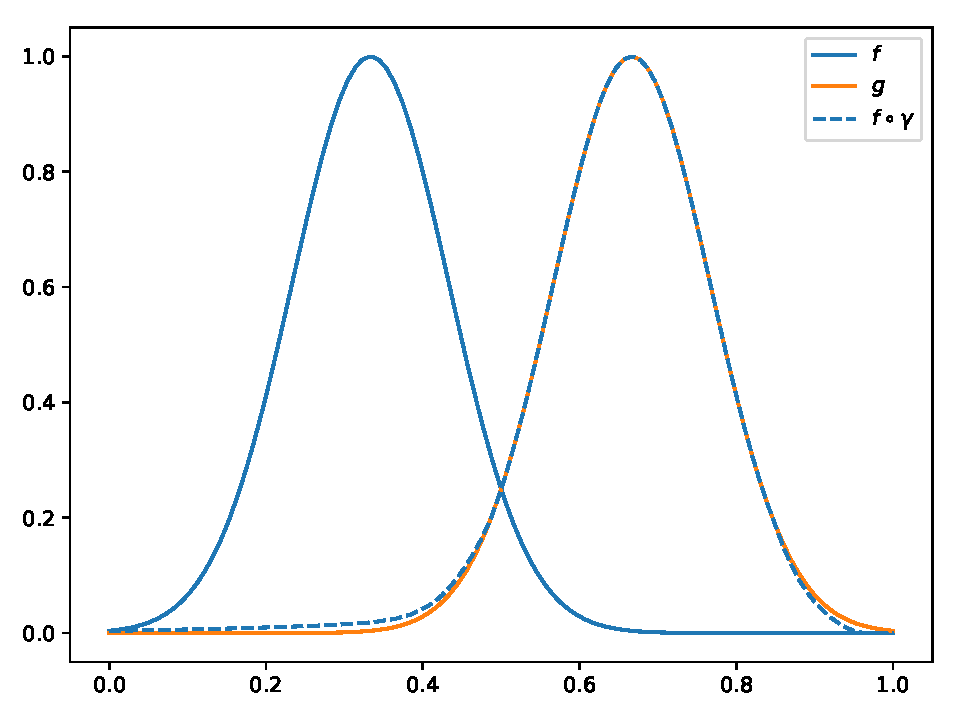
\includegraphics[width=7cm]{pairwise-alignment}} \quad
%  \subfigure[SBFIG:INVERSE1]{Alignment of $f_2$ to $f_1s$}{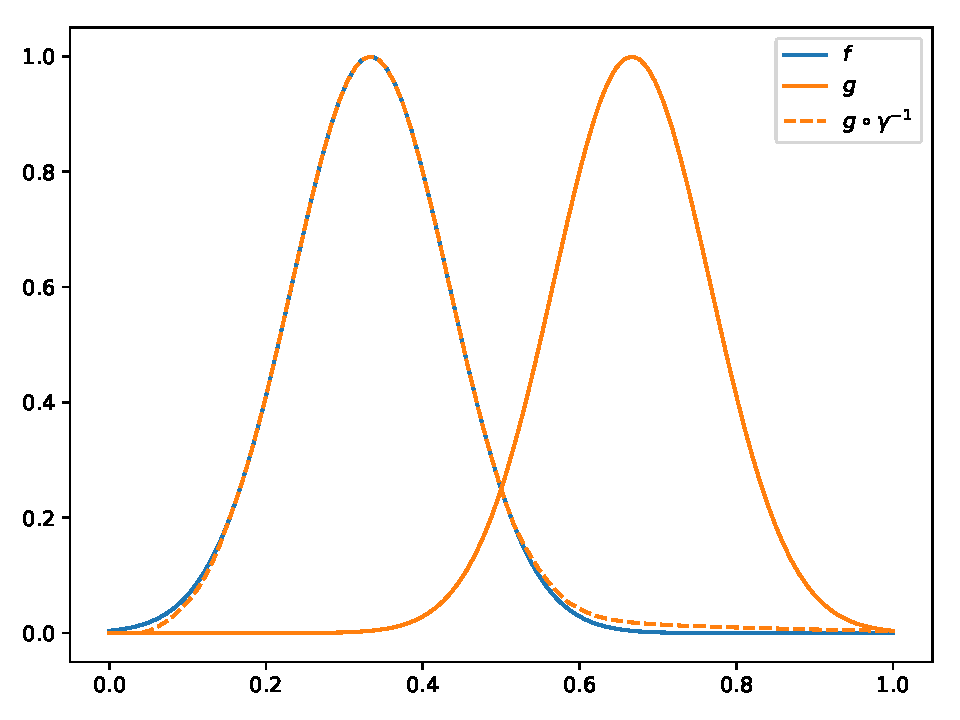
\includegraphics[width=7cm]{pairwise-alignment-inverse}}
%\end{figure}
